\documentclass[letterpaper, 11pt]{article}

\usepackage{lastpage, marginnote, siunitx, circuitikz, kantlipsum, hyperref, amsmath, circuitikz}
\def\UrlBreaks{\do\/\do-}

%\usepackage[hyphens]{url}

\usepackage{geometry}
\geometry{hscale=.6, vscale=.8, hmarginratio=2:1, vmarginratio=1:1, marginparwidth=.18\paperwidth, ignoremp}
%\geometry{marginparwidth=.1\paperwidth}

%\usepackage[T1]{fontenc}

\usepackage[explicit]{titlesec}
\titlespacing*{\section}{\dimexpr -\marginparsep-\marginparwidth}{*4}{*1}
\titleformat{\section}[runin]{\large\bfseries\titlerule[.5pt]\filright}{\makebox[1em][c]{\thesection}}{1em}{\parbox[t]{\dimexpr\marginparwidth-2em}{#1}\hskip\marginparsep\mbox{}}[\newline\vspace{-4ex}]

%\titlespacing*{\subsection}{\dimexpr -\marginparsep-\marginparwidth}{*4}{*1}
%\titleformat{\subsection}[runin]{\large\bfseries\titlerule[.5pt]\filright}{\makebox[1em][c]{\thesection}}{1em}{\parbox[t]{\dimexpr\marginparwidth-2em}{#1}\hskip\marginparsep\mbox{}}[\newline]

\usepackage{enumitem}
\newlist{steps}{enumerate}{1}
\setlist[steps]{label=Step \arabic*, font=\bfseries, leftmargin=-\marginparsep, itemindent=\marginparsep, align=right}

\usepackage{fancyhdr}
\pagestyle{fancy}
\fancyhf{}
\fancyhfoffset[lh,lf]{\dimexpr\marginparwidth+\marginparsep}
\fancyhf[lh]{UCD EEC 134}
\fancyhf[ch]{}
\fancyhf[rh]{}
%\fancyhf[lf]{left foot}
%\fancyhf[cf]{centre foot}
\fancyhf[rf]{Page \thepage /\pageref{LastPage}}
%\renewcommand{\footrulewidth}{.4pt}

%%%%%%%%%%%%%%%
%%%% Tikz definitions
%%%%%%%%%%%%%%%
%\tikzstyle{Uno}=[rectangle,fill=white,draw,line width=0.5mm]

%new commands
%display due date in red and link to the eec134-schedule.pdf document
\newcommand{\due}[1]{\href{https://github.com/ucdart/UCD-EEC134/blob/master/support/schedule/eec134-schedule.pdf}{\textcolor{red}{#1}}}

\graphicspath{{./figures/}}

\begin{document}

\title{Lab 4: Characterization of RF Mixers}
\author{Instructor: Xiaoguang ``Leo'' Liu\\lxgliu@ucdavis.edu \\
	\small \href{http://creativecommons.org/licenses/by-sa/4.0/}{CC BY-SA 4.0}}
\date{Last updated: \today}

\maketitle

In this lab, we will learn the techniques for characterizing high frequency mixers. 

%\section{Objectives}
%
%\begin{enumerate}[itemsep=0.1ex]
%	\item Learn how to characterize RF mixers.	
%\end{enumerate}

%Be warned that this lab is a fairly aggressive one and it will take a lot of time for you and your group to finish all the reading, the pre-lab assignment, the actual lab, and the reports. It's a good idea to start early! And divide up tasks between group members wisely!


\section{Deliverables}
All items are to be submitted through Canvas.  

\vspace{0.5cm}

\begin{table}[h]
	\footnotesize
	\caption{Lab 4 Deliverables}
	\renewcommand{\arraystretch}{1.2}
	\begin{tabular}{|m{1in}|l|m{0.45in}|m{2in}|}
		\hline
		\textbf{Item} & \textbf{Due date} & \textbf{Format} & \textbf{File name format} \\
		\hline
		\hline
		Pre-lab 4 & \due{Nov.~12th, 2017} & pdf & ``prelab-4-YourName.pdf''\\
				
		\hline
		Lab 4 report & \due{Nov.~19th, 2017} & pdf & ``lab-4-GroupName.pdf''\\
		\hline
	\end{tabular}
	\label{tab:deliverables}
\end{table}

\textbf{Notes:}
\begin{enumerate}
	\item All items are due by 11:59pm of the due date. No late submissions are accepted. Don't even ask. 
	
	\item Please follow the file name format rigorously. Replace ``GroupName'' with your group's name and ``YourName'' with your name, first name first, last name last. 
\end{enumerate}


\section{Prelab}
\begin{enumerate}
	\item Read the follow materials and pay close attention to the concepts of antenna \textit{conversion gain/loss}, \textit{LO drive}, \textit{LO feedthrough}, \textit{isolation}, \textit{image frequency},\textit{image rejection}, and \textit{quadrature modulation/demodulation}. 
	\begin{itemize}
		\item EEC 134 Lecture Note 5 
		
		\item Bert C.~Henderson, ``Mixers,'' WJ Communications Inc. technical notes, 1990. 
		\item Ferenc Marki and Christopher Marki, ``Mixer Basics Primer,'' Marki Microwave, 2010.
	\end{itemize}
	\item Read the Lab 4 procedures. 

\end{enumerate}


\reversemarginpar
\marginnote{\textbf{Pre-lab Assignment}\\\textbf{4} }

Please answer the following questions:
\begin{enumerate}
	\item What does ``Level 10'' mean in the specification of the Mini-Circuits ZX05-43LH-S+ mixer?
	
	\item What is the conversion gain/loss of the ADI ADL5363 mixer?
	
	\item What is the power conversion gain/loss of the ADI ADL5801 mixer? What is the voltage conversion gain/loss of this device? Why is there a difference between the power and voltage conversion gain/loss?
	
	\item What is the input IP3 of the Linear LTC5551 mixer? How does it compare with the ADI ADL5365 mixer?
	
	\item A 5.25\,GHz RF signal is fed to the input of a mixer driven by an LO signal of 5.20\,GHz. What signal do you expect at the output of the mixer?
	
	\item What are the image frequencies of the following systems?
	\label{pblm:image-freq}
		\begin{figure}[ht]
			\centering	
			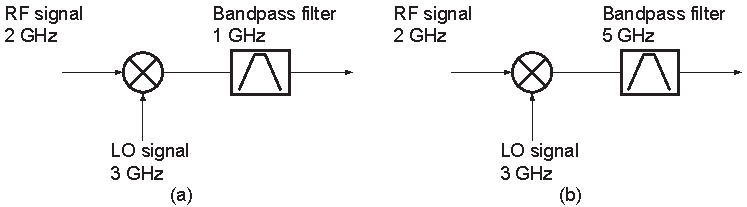
\includegraphics[width=4.5in]{image-freq}
			\caption{Prelab problem~\ref{pblm:image-freq}.}
			\label{fig:image-freq}
		\end{figure}
	
	\item What is the output signal frequency of the following system? Assume that $\omega_{IF} \ll \omega_{LO}$.
	\label{pblm:quad-freq}
	
		\begin{circuitikz}
			\draw (0,0) to (1,0) 
			(0,0) node[above]{$\cos \left( \omega_{IF}t \right)$}
			(1,-0.5) rectangle (3.3,0.5)
			(2.5, 0.5) to (2.5, 1.5) to (4,1.5)
			(4.5,1.5) node[mixer](mix){}
			(mix.in 2) node[below] {$\cos\left( \omega_{LO}t \right)$}
			(5, 1.5) to (6.5,1.5) to (6.5,0.5)
			(6,-0.5) rectangle (8.8,0.5)
			(2.5, -0.5) to (2.5, -1.5) to (4,-1.5)
			(4.5,-1.5) node[mixer](mix){}
			(mix.in 2) node[below] {$\sin \left( \omega_{LO}t \right)$}
			(5, -1.5) to (6.5,-1.5) to (6.5,-0.5)
			(1,0) node[right]{3\,dB splitter}
			(6,0) node[right]{power combiner}
			(8.8,0) to (9.8,0)
			(9.8,0) node[above]{?}
			;
		\end{circuitikz}
			
	\item What is the image reject ratio (side-band suppression) of the TI TRF370417 demodulator?
	
\end{enumerate}

\section{Equipment \& \\Supplies}

\begin{itemize}[itemsep=0.5ex]
	\item 1 $\times$ GSP-730 spectrum analyzer;
	\item 2 $\times$ TPI synthesizer;
	\item 1 $\times$ Mini-Circuit ZX05-43LH-S+ mixer;
	\item 2 $\times$ 12'' and 2 $\times$ 6'' SMA cables.
\end{itemize}

\section{Procedures}

\subsection{Mixer conversion loss}
\label{sec:mixer_cl}

\begin{enumerate}
	\item Connect the system based on the schematic shown in Fig.~\ref{fig:setup-mixer}.
	
		\begin{figure}[ht]
			\centering	
			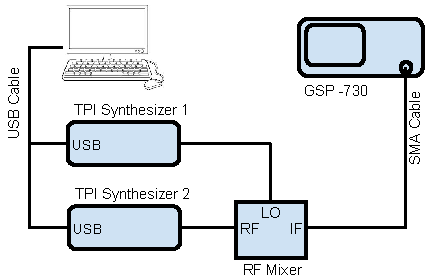
\includegraphics[width=3.5in]{setup-mixer}
			\caption{Mixer characterization setup.}
			\label{fig:setup-mixer}
		\end{figure}
	
	\item Set the output power of the first TPI synthesizer to 10\,dBm. 
	
	\item Set the output power of the second TPI synthesizer to 0\,dBm. 
	
	\item Power on the amplifier and spectrum analyzer. 
	
	\item Set the frequencies of the TPI synthesizers according to Table.~\ref{tab:freq} to investigate how the conversion-loss changes with frequency. The conversion loss can be calculated as 
	
	\[
		Conversion~Loss~\text{(dB)} = RF~Port~Power~\text{(dBm)} - IF~Port~Power~\text{(dBm)}.	
	\]
	
	\begin{table}[h]
		\centering
		\caption{RF and LO frequencies for mixer characterization.}
		\renewcommand{\arraystretch}{1.2}
		\begin{tabular}{|c|c|}
			\hline  RF Port Frequency (MHz) & LO Port Frequency (MHz)  \\ 
			\hline
			\hline  1000 & 1030  \\ 
			\hline  1500 & 1530 \\ 
			\hline  2000 & 2030 \\ 
			\hline  2500 & 2530 \\ 
			\hline  3000 & 3030 \\ 
			\hline  3500 & 3530  \\ 
			\hline  4000 & 4030 \\ 
			\hline 
		\end{tabular} 
		\label{tab:freq}
	\end{table}
	
\end{enumerate}

\subsection{LO Feed-through}

\begin{enumerate}
	\item Now we use the same setup as in Experiment.~\ref{sec:mixer_cl} to measure the LO feedthrough at different frequencies. Set the output power of the  first TPI synthesizer (the one connected to the LO port) to 10\,dBm. Turn off the second TPI synthesizer to block the RF port of the mixer. 
	
	\item Set the output frequency of the first TPI synthesizer from 1\,GHz to 3\,GHz in increment of 0.4\,GHz, and note down the measured IF port power. 

	\item Calculate the LO feedthrough at those frequencies by the following equation
	\[
		LO~Feedthrough~\text{(dB)} = IF~Port~Power~\text{(dBm)} - LO~Port~Power~\text{(dBm)}.
	\]
		How does the measurement compare with the datasheet of the mixer?
	
\end{enumerate}

\subsection{Mixer P1dB}

\begin{enumerate}
	\item Use the same setup as the previous experiments. Set output power and frequency of the first TPI synthesizer to 10\,dBm and 2500\,MHz. Set the output frequency of the second TPI synthesizer to 2530\,MHz. 

	\item Vary the output power of second TPI synthesizer and measure the IF output power of mixer at each input level. Choose the sample data points wisely (Note: the datasheet says the typical value of 1\,dB compression point is 9\,dBm). 

	\item Extract the P1dB of the mixer and compare it with the datasheet. 

\end{enumerate}


%\newpage
%\begin{thebibliography}{9}
%
% 
%\bibitem{thomas-sa}
%Jeff Thomas, Tom Holmes, Terri Hightower, ``Learn RF Spectrum Analysis Basics,'' Agilent Technologies, \url{https://www.jlab.org/uspas11/Reading/RF/RF%20Spectrum%20Analysis.pdf}.
%
%\bibitem{diez-sa}
%Erik Diez, ``The Fundamentals of Spectrum Analysis,'' Agilent Technologies, \url{http://electronicdesign.com/test-amp-measurement/fundamentals-spectrum-analysis}.
%
%
%\end{thebibliography}

\end{document}